%%%%%%%%%%%%%%%%%%%%%%%%%%%%%% -*- Mode: Latex -*- %%%%%%%%%%%%%%%%%%%%%%%%%%%%
%% 04-14.tex -- Thesis white paper - software inspections
%% Author          : Aaron A. Kagawa
%% Created On      : Mon Sep 23 11:52:28 2004
%% Last Modified By: Aaron Kagawa
%% Last Modified On: Wed Oct 27 15:16:41 2004
%% RCS: $Id$
%%%%%%%%%%%%%%%%%%%%%%%%%%%%%%%%%%%%%%%%%%%%%%%%%%%%%%%%%%%%%%%%%%%%%%%%%%%%%%
%%   Copyright (C) 2004 Aaron A. Kagawa
%%%%%%%%%%%%%%%%%%%%%%%%%%%%%%%%%%%%%%%%%%%%%%%%%%%%%%%%%%%%%%%%%%%%%%%%%%%%%%%
%% 

\documentclass[11pt,twocolumn]{article} 
\input{/export/home/csdl/tex/psfig/psfig}
\usepackage{/export/home/csdl/tex/icse2003/latex8}
\usepackage{times}
%% A verbatim-like environment which allows font changes
%%\usepackage{alltt}
%% New LaTeX2e graphics support
\usepackage[final]{graphicx}
% uncomment the % away on next line to produce the final camera-ready version
% and uncomment the \thispagestyle{empty} following \maketitle
\pagestyle{empty}

\begin{document}

\title{Determining What Code to Inspect and What Code Not to Inspect}

\author{\protect\begin{tabular}{ccc}
Aaron A. Kagawa \\
\end{tabular}\\
\em  Collaborative Software Development Laboratory \\
\em  Department of Information and Computer Sciences \\
\em  University of Hawai'i \\
\em  Honolulu, HI 96822 \\
\em  kagawaa@hawaii.edu}
\maketitle
\thispagestyle{empty}

\begin{abstract}  % 200 words
Imagine that your manager has scheduled 200 hours specifically for
conducting inspections. However, you realize that you actually need 400
hours to adequately inspect the majority of the system.  How do you make
a distinction between what documents need to be inspected and the
documents have to be skipped?
  
This hypothetical situation is not as uncommon as one would think. Yet, the
classical definition of inspections does not provide any advice on how to
handle this very common problem. More specifically, the notion of entry
criteria used in Software Inspections determines if documents are ready for
inspection \cite{Ebenau94} rather than if inspections are needed at all.

This research investigates whether we can apply the hypothetically
available 200 hours of inspection to areas of the system that need it most.
It is commonly accepted that eighty percent of the defects in a system come
from twenty percent of the system \cite{Boehm01}. The ideal situation is to
apply the 200 hours directly to that twenty percent.

To accomplish this, I hypothesize that it is possible for quality measures
to distinguish documents that are in ``most need of inspection'' from those
in ``least need of inspection''. In some sense it flips the adage of ``the
process of inspection leads to an increase of quality'' to ``an
understanding of quality will make inspection more cost effective''. It is
my claim that this determination will help project managers to focus their
inspections to critical areas of the system.
\end{abstract}

\Section{Introduction}
\label{sec:intro}
The use of software inspections has reported outstanding results in
improved productivity and quality. In fact, one study has found that if the
inspection process is followed correctly, then up to 95 percent of defects
can be removed before entering the testing phase \cite{Bush90}.
Inspections have been so successful that it is likely to be the closest
thing we have to a ``silver bullet'' for improving software quality.

%%Since the introduction of inspections by Michael Fagan, there have been
%%numerous views, descriptions, and process that have been proposed by
%%various authors and researchers. Some of these include; Fagan Inspections
%%\cite{Fagan76}, Software Inspections \cite{Gilb93}, High-Impact
%%Inspections, and Phased Inspections just to name a few. Throughout this
%%paper I will use the lower cased inspection to represent all inspection
%%techniques.

In another success story, the Jet Propulsion Laboratory adopted inspections
to identify defects and experienced a savings of 7.5 million dollars by
conducting 300 inspections \cite{Bush90a}. This statistic is very
impressive, however what is not usually emphasized is that each inspection
had an average cost of 28 hours. Using that average cost, the total cost
for JPL's inspection process was 8,400 hours or roughly 4 years of work.
This illustrates a fundamental problem with inspections; better results
come from better investment \cite{Gilb93}.

Not all organizations have the time or the money to fully invest into
inspections. In most cases, organizations have limited funds or resources
that can be devoted to inspections. For example, a manager can devote 200
hours of a project schedule for inspections. These organizations must pick
and choose what documents to use those precious resources on.  This
realistic management of inspections directly contradicts the classical
inspection adage of ``when a document is ready you should inspect it''. The
bottom line is that most organizations cannot inspect every document.

The correct inspection process begins with the initiation phase, or
sometimes called the planning stage, in which authors volunteer their
documents for inspection \cite {Gilb93}. The inspection leader then checks
the document against entry criteria to determine if the document is ready
for inspection \cite{Ebenau94} \cite{Gilb93}. Again this process works very
well for organizations, like JPL, that have the resources to inspect every
document that is ready. However, I believe that this phase of inspection is
a major problem for organizations that do not the necessary resources,
because the process does not consider that some documents are ``better'' to
inspect than others. A simple illustration of this fact is that 80 percent
of defects come from 20 percent of the modules \cite{Boehm01}.  Thus,
volunteering a document from that 20 percent will likely be ``better'' than
in any other module.

Furthermore, the current literature \cite{Ebenau94} \cite{Wiegers02}
\cite{Gilb93} on inspections does not provide any specific insights into
the trade offs between inspecting some documents and not inspecting others.
However, Tom Gilb provides two recommendations when resources are limited;
sampling and emphasizing inspecting up-stream documents \cite{Gilb93}. The
use of sampling involves inspecting various areas of a system to identify
areas of interest. Up-Stream documents are documents that define high-level
requirements or designs. The idea is that at the very least we should
ensure that high-level documents are of high quality. Although, these are
very useful recommendations, they do not provide much specific guidance of
how best to use limited resources. At the end of the day, an organization
with limited inspection resources must select documents to inspect. 

The goal of this research is to optimize the selection of documents for
inspection. To do this I will create a Hackystat extension that will
determine what packages are in ``most need of inspection'' versus packages
that are in ``least need of inspection''. There are several research
questions that I must answer in order to make that determination. The most
important question is the operational definition of the general terms
``most need'' and ``least need''. What software attributes can quantifiably
distinguish between ``most'' and ``least'' need of inspection? In order to
create a definition we must understand the motivation for inspections.

Software inspection has two primary goals; increase quality and
productivity. For this research I am primarily concerned with increasing
quality. The successful inspection of a document has two main results:
finding defects which, once removed, increases software quality or not
finding defects thus indicating high software quality. Software quality is
vaguely defined as ``the degree to which software possess a desired
combination of attributes'' \cite{IEEEGlossary83}. Some of the possible
attributes can include: portability, reliability, efficiency, usability,
testability, understandability, and modifiability \cite{Glass03}. Some
other widely accepted measures of quality include defect density and
complexity.  Whatever definition used for quality, inspections aim to
increase or validate the level of quality in software. Therefore, I would
claim that the same attributes defining software quality also provide good
indications of what code to inspect. For example, finding code that has low
portability, reliability, efficiency, usability, testability,
understandability, and modifiability would be a good indication of code
that would be beneficial to inspect.

My thesis claim is as follows: 
\begin{enumerate}
\item The attributes that define software quality provide good indications
  of what code to inspect.
\item Code that represents ``high'' software quality will have a low number
  of defects found in inspection.
\item Code that represents ``low'' software quality will have a high number
  of defects found in inspection.
\end{enumerate}

\Section{Evaluation Methodology}
\label{sec:evaluation}
To evaluate my thesis claims, I will create a Hackystat Extension that will
determine what packages are in ``most need of inspection'' from `packages
that are in ``least need of inspection''. When the system makes a
determination of what package is in most need of inspection, I will
recommend a package for inspection. The results of the inspection (i.e.
number of critical issues) will determine if the package accurately
reflects the ``most'' and ``least'' need of inspection determination.  To
do this, I first need to gain a basic understand of the attributes that
affect quality.

It is important to note that I am not defining a set of attributes that
represent quality for all software projects. Instead, by using the
Hackystat Extension I will be able to go through a methodology to best
calibrate the attributes to accurately reflect the quality for the project
that I am studying.

For this evaluation, I will study the implementation of the Hackystat
System developed in the Collaborative Software Development Laboratory, of
the University of Hawaii at Manoa. Although, this is a project to which I
also contribute, I will minimize any possible data contamination by doing
two things. First, I will keep the results of the ``most'' and ``least''
need of inspection a secret both during and after conducting the
inspection. Second, I will not participate in the inspections themselves.

To evaluate claim 1, I will conduct several weekly mini-studies to
fine-tune my calculation of quality. I will begin my study with several
basic attributes defined in the literature that are believed to affect
quality. Some of these attributes include size and coverage. Based on the
quality level, I will then recommend a specific package for inspection by
the CSDL staff. After the inspection, I will analyze the number of valid issues
generated and their severity. Thus, I will be able to conclude if the
quality level actually reflected a package that was in most need of inspection.
I will continue to fine-tune the attributes of quality on a weekly basis.
Once I have verified the attributes of quality, I can begin to evaluate
claim 2 and 3.

To evaluate claim 2 and 3, I will recommend and collect data on the
inspections for a 6-week period. During this period, I will specifically
choose three high quality and three low quality packages. If my selected
attributes are correct then the high quality packages should have
considerably less issues generated by inspection than the low quality
packages.

\Section{Hackystat Quality Extension}
This section provides a short description of the Hackystat Quality
Extension system. This system extends the functionality of the Hackystat
System to provide the ``most'' and ``least'' need of inspection determinations.

The Hackystat System provides several Sensor Data Types that represent
quantitative data about both the product and development process of a
software project. Using this data I will build attributes that represent
quality. For example, some of the attributes that are currently possible
are the following:

\begin{enumerate}
\item Active Time
\item Number of Changes (Commits)
\item Date of Last Change
\item Number of Inspections
\item Date of Last Inspection
\item Number of Defects
\item Date of Last Defect
\item Lines of Code, Number of Methods, and Number of Classes
\item Lines of Test Code, Number of Test Methods, and Number of Test
Classes
\item Coverage
\end{enumerate}

Currently, each of these attributes is collected for each package or
workspace within a specified project. Figure 1 shows several example high
quality (or ``least need of inspection'') workspaces with their respective
attributes of quality.

\begin{figure*}[ht]
  \centering
  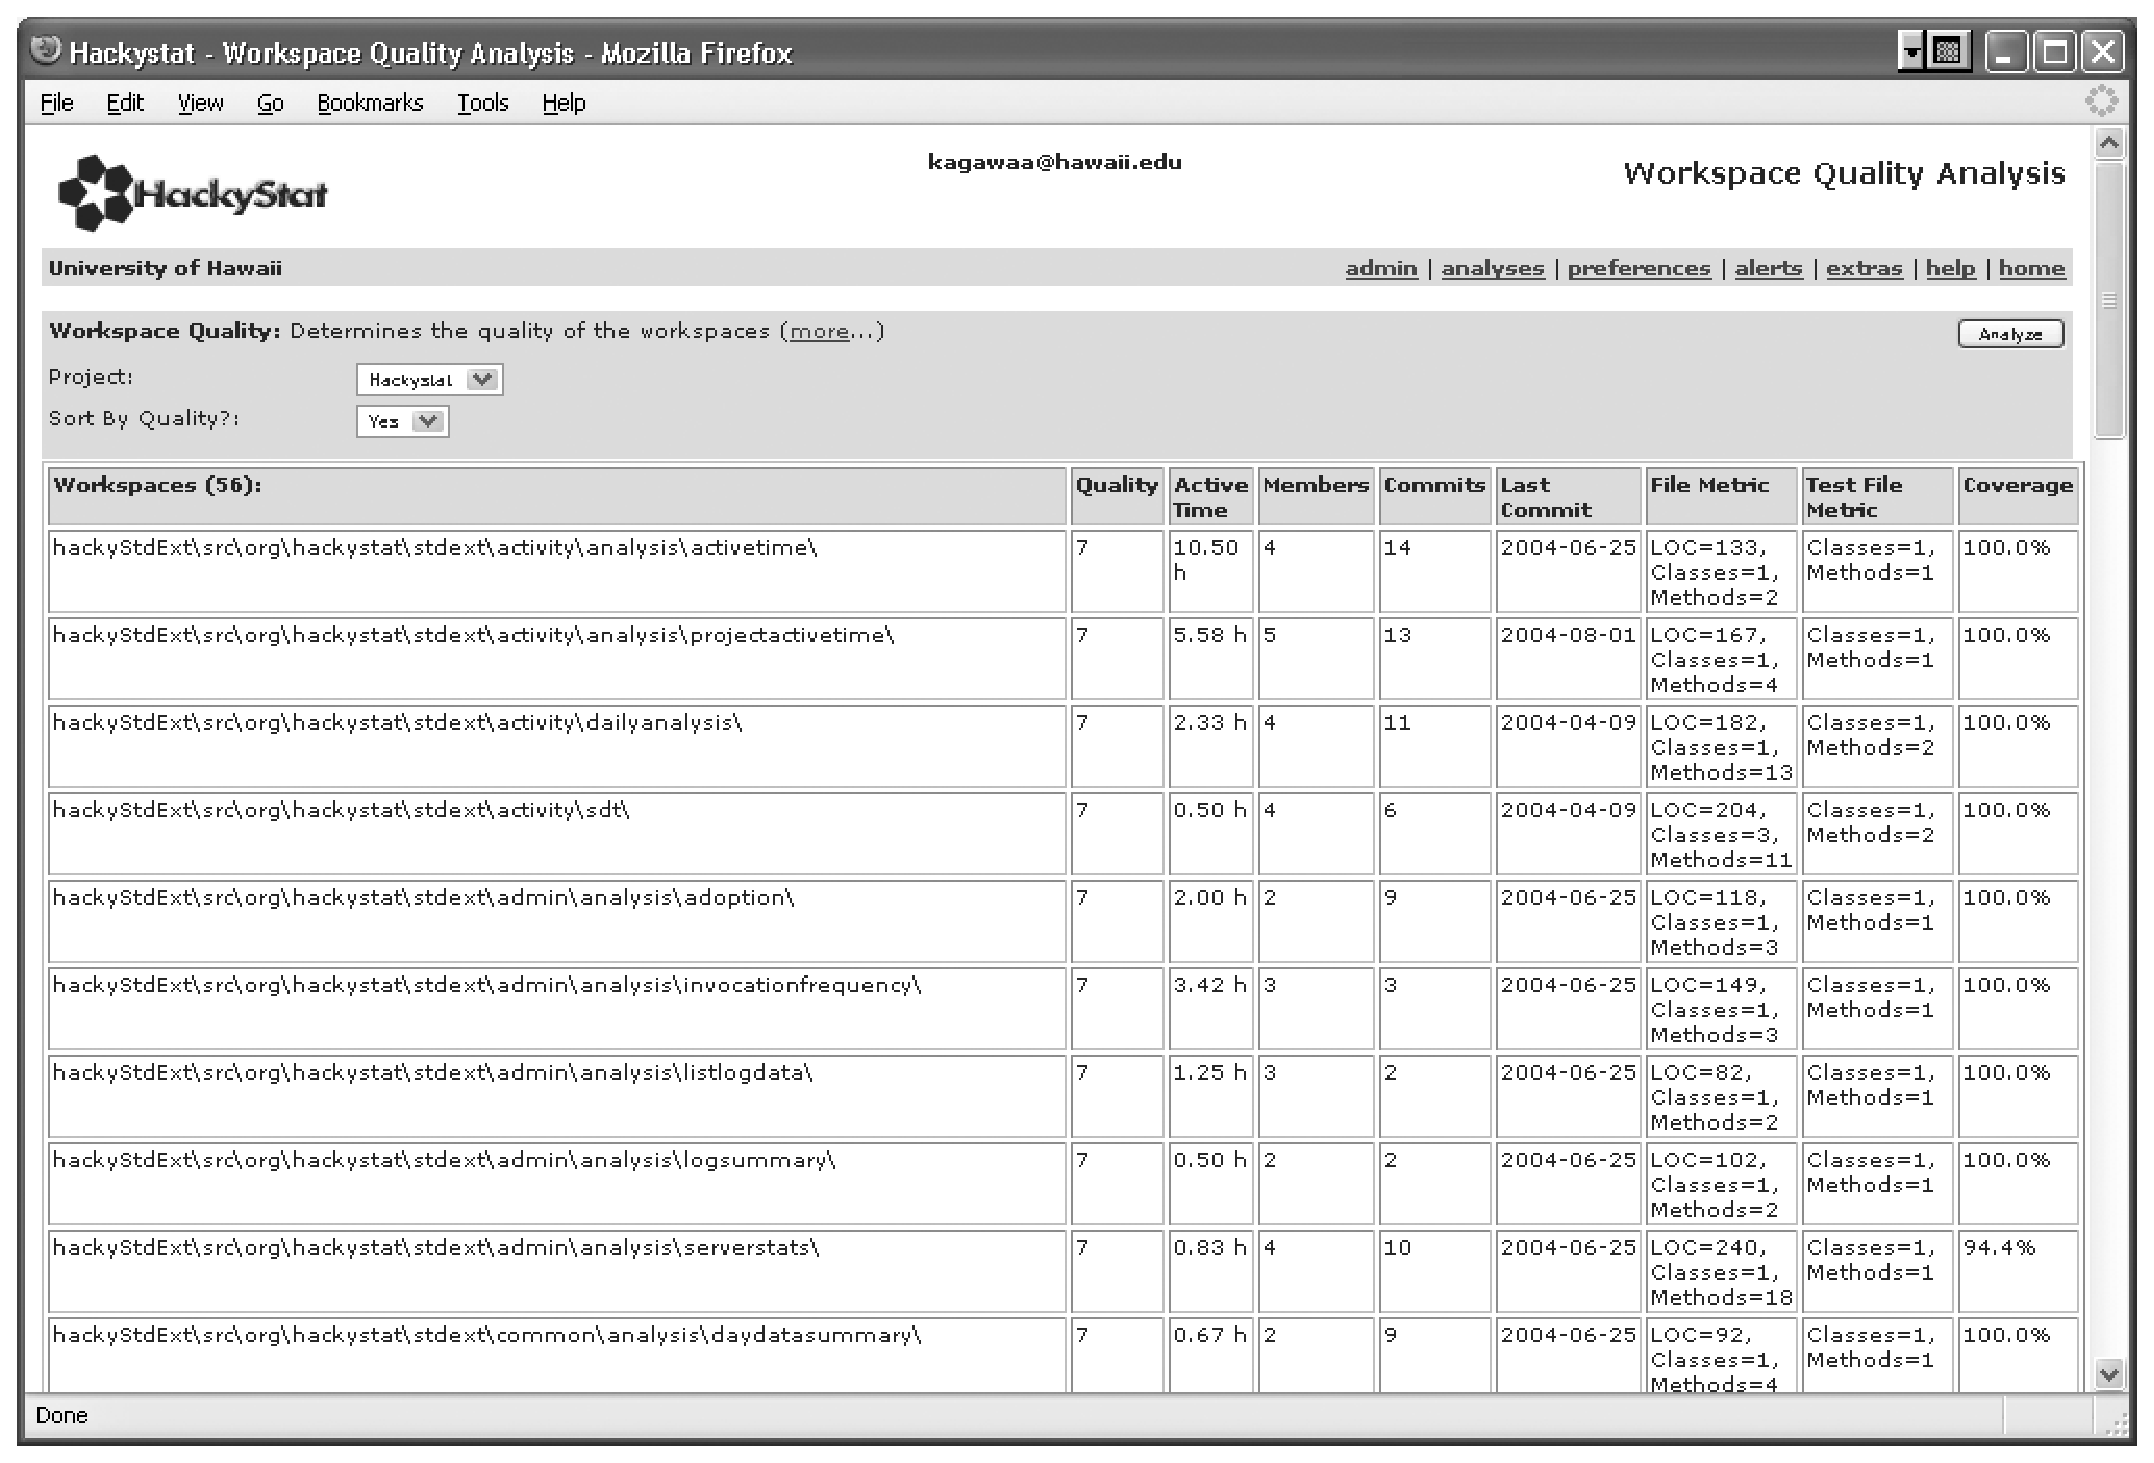
\includegraphics[width=1.00\textwidth]{WorkspaceQuality.eps}
  \caption{The Workspace Quality analysis. Workspaces are listed with its
  respective quality level and the attributes that make up its quality
  level.
}
  \label{fig:WorkspaceQualityAnalysis}
\end{figure*}

To make the important determination of ``most'' and ``least'' need of
inspection, I assign certain quality levels or numerical weights to the
attributes. For example, if the coverage of a package is below 80 percent,
I assign a ``low'' quality level for that attribute. Likewise, if the
coverage of a package is a 100 percent, then I assign a ``high'' quality
level. ``Low'' is operationalized by a 1, ``high'' is operationalized by a
3, and ``middle ground'' is operationalized by a 2. The system assigns each
attribute a quality level and then assigns each package an aggregated
quality level, which is the sum of the quality levels associated with its
attributes. The packages are then sorted by the packages' aggregate quality
level, sorting the ``most need of inspection'' to the bottom and ``least need
of inspection'' to the top.

There are several issues with the assignment of numerical weights (or
quality levels as I call them) that I still need to address. For example, I
explicitly determine the quality levels using my own subjective measure of
what is low versus high quality. I will need to explore if my subjective
measure is sufficient, if some attributes should be weighted more than
others, or if any other entirely different weighting methods provide more
accurate results.

\Section{Initial Results}
The use of the Hackystat Quality Extension system to provide the
determination of ``most'' and ``least'' need of inspection has been promising.
The initial implementation of the system has proven that it is technically
possible to do what I have envisioned. In addition, I have already
recommended the inspection of a package that was in ``most need of a inspection''
and the defects and issues identified have confirmed that the package had
low quality.

Of course, I will continue to discover new attributes to define quality,
fine tune the numerical weights associated with the attributes, and
continue to recommend inspections until I believe my mechanism is ready for a
thorough evaluation.

\Section{Contributions}
If I find evidence that my thesis claims are true, then I believe the
formal inspection process should address some sort of quantitative approach
for initiating inspections.

In addition, I believe that the system's quantification of quality is
valuable in of itself. Development teams can use the system's attributes of
quality to guide the management of quality.

\bibliographystyle{/export/home/csdl/tex/icse2003/latex8}
\bibliography{/export/home/csdl/techreports/04-14/04-14,/export/home/csdl/bib/csdl-trs,/export/home/csdl/bib/hackystat,/export/home/csdl/bib/ftr}
\end{document}




